%!TEX program = xelatex
% Encoding: UTF8
% SEIKA 2015


% Chapter 2 Tutorials
% Section 2.5


\newpage
\section {卷积神经网络} \label{cnn}

\subsection {Overview \footnote{This tutorial is intended for advanced users of TensorFlow and assumes expertise and experience in machine learning}}

CIFAR-10 classification is a common benchmark problem in machine learning. The problem is to classify RGB 32x32 pixel images across 10 categories: airplane, automobile, bird, cat, deer, dog, frog, horse, ship, and truck.

对CIFAR-10 数据集的分类是机器学习中一个公开的基准测试问题,其任务是对一组32x32RGB的图像进行分类,这些图像涵盖了10个类别:\lstinline{airplane}, \lstinline{automobile}, \lstinline{bird}, \lstinline{cat}, \lstinline{deer}, \lstinline{dog}, \lstinline{frog}, \lstinline{horse}, \lstinline{ship}, 和 \lstinline{truck}.

\begin{center}
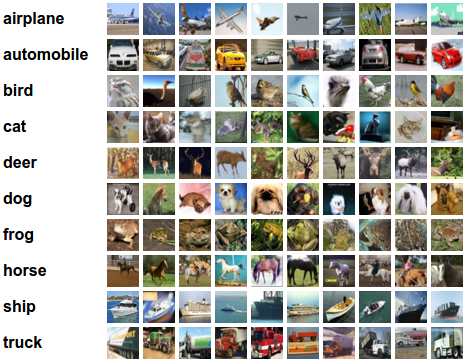
\includegraphics[width=.55\textwidth]{../SOURCE/images/cifar_samples.png}
\end{center}

想了解更多信息请参考\href{http://www.cs.toronto.edu/~kriz/cifar.html}{CIFAR-10 page},以及Alex Krizhevsky写的\href{http://www.cs.toronto.edu/~kriz/learning-features-2009-TR.pdf}{技术报告}。

\subsubsection {G目标}
本教程的目标是建立一个用于识别图像的相对较小的卷积神经网络,在这一过程中,本教程会:

\begin{itemize}
\item 着重于建立一个规范的网络组织结构,训练并进行评估;
\item 为建立更大规模更加复杂的模型提供一个范例
\end{itemize}

选择CIFAR-10是因为它的复杂程度足以用来检验TensorFlow中的大部分功能,并可将其扩展为更大的模型。与此同时由于模型较小所以训练速度很快,比较适合用来测试新的想法,检验新的技术。

\subsubsection {本教程的重点}
CIFAR-10 教程演示了在TensorFlow上构建更大更复杂模型的几个种重要内容:

\begin{itemize}
\item 相关核心数学对象,如卷积、修正线性激活、最大池化以及局部响应归一化;
\item 训练过程中一些网络行为的可视化,这些行为包括输入图像、损失情况、网络行为的分布情况以及梯度;
\item 算法学习参数的移动平均值的计算函数,以及在评估阶段使用这些平均值提高预测性能;
\item 实现了一种机制,使得学习率随着时间的推移而递减;
\item 为输入数据设计预存取队列,将磁盘延迟和高开销的图像预处理操作与模型分离开来处理;
\end{itemize}

我们也提供了模型的多GUP版本,用以表明:

\begin{itemize}
\item 可以配置模型后使其在多个GPU上并行的训练
\item 可以在多个GPU之间共享和更新变量值
\end{itemize}

我们希望本教程给大家开了个头,使得在Tensorflow上可以为视觉相关工作建立更大型的Cnns模型

\subsubsection {模型架构}

本教程中的模型是一个多层架构,由卷积层和非线性层(nonlinearities)交替多次排列后构成。这些层最终通过全连通层对接到softmax分类器上。这一模型除了最顶部的几层外,基本跟Alex Krizhevsky提出的模型一致。

在一个GPU上经过几个小时的训练后,该模型达到了最高86\%的精度。细节请查看下面的描述以及代码。模型中包含了1,068,298个学习参数,分类一副图像需要大概19.5M个乘加操作。

\subsection {Code Organization}

本教程的代码位于\href{https://tensorflow.googlesource.com/tensorflow/+/master/tensorflow/models/image/cifar10/}{tensorflow/models/image/cifar10/}.

% insert table here

\subsection {CIFAR-10 模型}


\subsubsection {Model Inputs}

\subsubsection {Model Prediction}

\subsubsection {Model Training}

\subsection {Lauching and Training the Model}

\subsection {Evaluating a Model}

\subsection {Traning a Model Using Multiple GPU Cards}

\subsubsection {Placing Variables and Operations on Devices}

\subsubsection {Lauching and Training the Model on Multiple GPU cards}

\subsection {Next Steps}



